\documentclass[10pt]{article}
\author{JS LAOSHI}


\usepackage{mathrsfs}

%\usepackage{amssymb,amsthm,amsmath,amssymb,latexsym,amsfonts,txfonts, pxfonts,wasysym,stmaryrd}
\textheight=230mm \textwidth=140mm
\topmargin=-1.5cm
\oddsidemargin=1.2cm
\evensidemargin=1.2cm
\setlength\parindent{0pt}
\parskip=7pt
%\setcounter{page}{1}
%\setlength{\baselineskip}{24pt} \baselineskip=24pt
\usepackage{amsmath,amsthm,amssymb}
\usepackage{graphicx}
\usepackage{bbm}
\usepackage{xcolor}
\usepackage[utf8]{inputenc}
\usepackage[english]{babel}
\usepackage{enumitem}
\usepackage{hyperref}
\usepackage{color}
\usepackage{colortbl}
\usepackage{tikz}
%\usepackage{vector}

\hypersetup{
    colorlinks=true,
    linkcolor=blue,
    filecolor=magenta,      
    urlcolor=cyan,
    pdftitle={Sharelatex Example},
    citecolor=red,
    % bookmarks=true,
}


\font\tencmmib=cmmib10 \skewchar\tencmmib '60
\newfam\cmmibfam
\textfont\cmmibfam=\tencmmib
\def\Ph{\mathchar'4010}
\def\Ps{\mathchar'4011}
\font\tensmc=cmcsc10
\def\smc{\tensmc}
\def\srm{\sevenrm }
\font\tenmsb=msbm10
\font\eightmsb=msbm10 scaled 1100
\def\Bbb#1{\hbox{\tenmsb#1}}
\def\Bbbb#1{\hbox{\eightmsb#1}}
\def\bbox{\quad\hbox{\vrule \vbox{\hrule \vskip2pt \hbox{\hskip2pt
\vbox{\hsize=1pt}\hskip2pt} \vskip2pt\hrule}\vrule}}
\def\lessim{\ \lower4pt\hbox{$
\buildrel{\displaystyle <}\over\sim$}\ }
\def\gessim{\ \lower4pt\hbox{$\buildrel{\displaystyle >}
\over\sim$}\ }
\def\n{\noindent}
\def\P{{\cal P}}
\def\si{\bar{\sigma}}
\def\E{{\cal E}}
\def\LL{{\cal L}}
\def\FF{{\cal F}}
\def\SS{{\cal S}}
\def\C{{\cal C}}
\def\D{{\cal D}}
\def\H{{\cal H}}
\def\X{{\cal X}}
\def\Y{{\cal Y}}
\def\A{{\cal A}}
\def\B{{\cal B}}
\def\O{{\cal O}}
\def\M{{\cal M}}
\def\I{{\cal I}}
\def\eps{{\varepsilon}}
\def\ch{{\mbox{\rm ch}\hspace{0.4mm}}}
\def\sh{{\mbox{sh}}}
\def\th{{\mbox{th}}}
\def\Av{{\mbox{\rm{Av}}}}
\def\n{\noindent}
\def\bbe{\vskip .15pc\hangindent=.5pc\hangafter=1}
\def\goin{\to\infty}
\def\qed{\hfill\break\rightline{$\bbox$}}



\newcommand{\e}{\mathbb{E}}
\newcommand{\p}{\mathbb{P}}
\newcommand{\lra}{\leftrightarrow}
\newcommand{\nlra}{\nleftrightarrow}
\newcommand{\bet}{\begin{theorem}}
\newcommand{\ent}{\end{theorem}}
\newcommand{\Var}{\mathrm{Var}}
\newcommand{\g}{\Gamma}
\newcommand{\de}{\delta}
\newcommand{\norm}[1]{\left\lVert#1\right\rVert}
\newcommand{\gy}[1]{\textbf{\color{red}[Yi: #1]}}
\newcommand{\olsi}[1]{\,\overline{\!{#1}}}
\newcommand\y{\cellcolor{blue!20}}
\newcommand\x{\cellcolor{red!20}}
\DeclareMathOperator{\Tr}{Tr}

\newtheorem{lemma}{\bf Lemma}
\newtheorem{claim}{\bf Claim}
\newtheorem{definition}{\bf Definition}
\newtheorem{theorem}{\bf Theorem}
\newtheorem{corollary}{\bf Corollary}
\newtheorem{remark}{\bf Remark}
\newtheorem{example}{\bf Example}
\newtheorem{exercise}{\bf Exercise}
\newtheorem{proposition}{\bf Proposition}
\newtheorem{question}{\bf Question}
\newtheorem{acknowledgements}{\bf Acknowledgements}

\newenvironment{Proof of lemma}{\noindent{\bf Proof of Lemma}}{\hfill$\Box$\newline}
\newenvironment{Proof of claim}{\noindent{\bf Proof of claim}}{\hfill$\Box$\newline}
\newenvironment{Proof of theorem}{\noindent{\bf Proof of Theorem}}{\hfill\scriptsize{$\Box$}\newline}
\newenvironment{Proof of theorems}{\noindent{\bf Proof of Theorems}}{\hfill$\Box$\newline}
\newenvironment{Proof of proposition}{\noindent{\bf Proof of Proposition}}{\hfill$\Box$\newline}
\newenvironment{Proof of propositions}{\noindent{\bf Proof of Propositions}}{\hfill$\Box$\newline}
\newenvironment{Proof of exercise}{\noindent{\it Proof of Exercise:}}{\hfill$\Box$}
\newenvironment{Acknowledgements}{\noindent{\bf Acknowledgements}}




\numberwithin{equation}{section}



\begin{document}


\title{Generalized m-Local Optimum of the Sherrington-Kirkpatrick Spin Glass Model}
\maketitle

\section{Introduction} \label{sec_intro}
Let $W = (W_{i,j})_{N\times N}$ be a symmetric matrix with zero diagonal such that $(W_{i,j})_{1 \leq i < j \leq N}$ are independent standard normal Gaussians. The \textit{Sherrington-Kirkpatrick} Spin Glass Model (a.k.a. the SK Model) is defined by its Hamiltonian, a random function $H:\{-1,+1\}^N \to \mathbb{R}$. To be precise,
\begin{align}
    H(\sigma) := \sum_{1 \leq i < j \leq N} \sigma_i \sigma_j W_{ij},
\end{align}
where $\sigma = (\sigma_i)^n_{i=1} \in \{-1,+1\}^n$ is called the spin configuration. Normally the Hamiltonian will come with a normalization factor in front of the summation. We will see very soon that in this paper we do not need such normalization. The value of the Hamiltonian $H(\sigma)$ evaluated at a specific configuration $\sigma$ is called the energy of the configuration $\sigma$.

The energy landscape of spin glass models has been a vital research topic in the field of mathematical physics. L. A-Berry et al. studied the probability of a configuration being local optimal in \cite{SK_optimal}. We plan to generalize the result. For the remaining of the section, we will establish the generalized concept of local optimum, give a quick debrief of the original approach in \cite{SK_optimal}, and why extending the result is difficult.

Intuitively speaking, a local optimal configuration $\sigma$ satisfies that taking any single step from it will cause the energy to increase. Indeed, for $i \in [N]:= \{1,\cdots, N\}$, define $\sigma^{(i)}$ to be
\begin{align}
    \sigma^{(i)}_j = 
    \begin{cases}
        \sigma_j&,  \text{if $j \neq i$} \\
        -\sigma_i&,  \text{if $j = i$}.
    \end{cases}
\end{align}
$\sigma$ is said to be a local optimum (\cite{SK_optimal}) if for any $i \in [N]$,
\begin{align}
    H(\sigma^{(i)}) \geq H(\sigma).
\end{align}
Every time we flip a single coordinate, we take a single step away from our starting point. This concept can easily be extended for scenarios where we take $m$ steps from $\sigma$, namely flipping $m$ coordinates. $m$ is a fixed positive integer. We also care about the configurations that will remain optimal if we take any steps(flips) from it as long as the number of steps(flips) is no larger than $m$. Since we always let $N \to \infty$ at the end, we don't have to worry about the cases that $m > N$. Below are the formal definitions:
\begin{definition} \label{mlo_def}
    Let $S$ be a subset of $[N]$. Define $\sigma^{(S)}$ to be
    \begin{align}
        \sigma^{(S)}_j = 
        \begin{cases}
            \sigma_j&,  \text{if $j \notin S$} \\
            -\sigma_j&,  \text{if $j \in S$}.
        \end{cases}
    \end{align}
    A configuration $\sigma$ is said to be an $m$-flip optimum if for any $S \subset [N]$, $|S|=m$,
    \begin{align}
        H(\sigma^{(S)}) \geq H(\sigma).
    \end{align}
    Moreover, a configuration $\sigma$ is said to be an $m$-optimum if for any $S \subset [N]$, $|S|\leq m$,
    \begin{align}
        H(\sigma^{(S)}) \geq H(\sigma).
    \end{align}
\end{definition}
In \cite{SK_optimal}, the computation starts by introducing a group of Gaussian random variables
\begin{align}
    Z_i := \frac{H(\sigma^{(i)}) - H(\sigma)}{2} , \forall i \in [N].
\end{align}
Clearly, $\sigma$ is a local optimum if and only if $Z_i \geq 0$ for all $i \in [N]$. And from here we can easily see that the normalization factor doesn't matter. Also,
\begin{align}
    Z := (Z_1,\cdots Z_N)^T
\end{align}
is a multivariate Gaussian vector with zero mean. Denote $C$ its covariance matrix, and we have
\begin{align} \label{lo_original}
    &\p(\text{\normalfont $\sigma$ is local optimal}) = \p(Z_i \geq 0, \forall i \in [N]) \nonumber \\
    =&\frac{1}{(2\pi)^{N/2}det(C)^{1/2}}\int_{[0,\infty)^N} \exp \left(\frac{-x^T C^{-1} x}{2}\right)dx.
\end{align}
The rest is to compute $C^{-1}$ (which is not hard), and do asymptotic analysis using large deviation theory(\cite{SK_optimal}). It is worth remarking that the computation shows the covariance matrix $C$ does not depend on our choice of configuration $\sigma$, and so is the probability.

The story becomes different for $m$-flip local optimum (and in turn, $m$-optimum). Likewise, we define for any $S \subset [N]$, $|S|=m$,
\begin{align} \label{zs_formula}
    Z_S := \frac{H(\sigma^{(S)})- H(\sigma)}{2}.
\end{align}
Then $\sigma$ is an $m$-flip local optimum if and only if $Z_S \geq 0$ for all $m$-subsets $S \subset [N]$. We can write down the probability of $m$-flip local optimum in the same way as we did in (\ref{lo_original}). However, instead of getting an $N$-by-$N$ covariance matrix, we will get a $\binom{N}{m}$-by-$\binom{N}{m}$ covariance matrix, which is much larger, and turns out to be much complicated than the original one. Understanding the new covariance matrix and its inverse becomes the core of our work.

\section{Layout of the Paper} \label{sec_layout}
To give the readers a clearer picture, we dedicate this short section to give a summary of each section's content.

In section \ref{sec_result}, we will state the main theorem for quick reference and introduce some frequently used notations.

In section \ref{sec_covariance}, we will compute the covariance matrix for $m$-flip local optimum and show it also does not depend on our choice of $\sigma$. A quick example of $2$-flip covariance structure will be provided for better intuition and illustration.

In section \ref{sec_inverse}, we will investigate the properties of the covariance matrix, and compute its inverse.

In section \ref{sec_integral}, we will do asymptotic analysis of the integral that gives us the probability of local optimum, and establish a large deviation principle (LDP).
\section{Main Results} \label{sec_result}
Under Construction.
\section{Covariance Structure} \label{sec_covariance}
Let $Z_S$ be defined as in (\ref{zs_formula}). We will start this section by computing the covariance structure of $2$-flip as an example. And we will see later that though for $m$-flip covariance structure there are daunting amount of indices, the pattern and the deduction method are no different from those of $2$-flip.
\begin{example} \label{2_flip_covar_example}
    Let $\{a,b\}$ be an arbitrary 2-subset of $[N]$. Let $H(\sigma^{(\{a,b\})})$ be defined as in definition \ref{mlo_def}, we consider 
    \begin{align}
        Z_{\{a,b\}}:=\frac{H(\sigma^{(\{a,b\})}) -H(\sigma)}{2}.
    \end{align}
    Recall that
    \begin{align}
        H(\sigma) := \sum_{1 \leq i < j \leq N} \sigma_i \sigma_j W_{ij}.
    \end{align}
    If neither $i$ nor $j$ belongs to $\{a,b\}$, the term $\sigma_i \sigma_j W_{ij}$ will stay the same and not appear in the formula of $Z_{\{a,b\}}$. On the other hand, if $\{i,j\} = \{a,b\}$, the term $\sigma_a \sigma_b W_{ab}$ will also stay the same because both $\sigma_a$ and $\sigma_b$ are flipped. Finally, $i \neq j$ for all $i,j$ by definition. Therefore, we obtain
    \begin{align} \label{2flip_z_formula}
        Z_{\{a,b\}} = - \sum_{j \neq a, j \neq b} \sigma_a \sigma_j W_{a,j} - \sum_{j \neq a, j \neq b} \sigma_j \sigma_b W_{j,b}.
    \end{align}
    Now we can compute the covariance. Let $\{s_1,s_2\}$ and $\{t_1,t_2\}$ be two sets of flipped coordinates. We divide our computation into several cases.

    \textbf{Same Flip} ($s_1 = t_1 = a, s_2 = t_2 =b $ for some $a,b$.) In this case, we rewrite
    \begin{align}
        Z_{\{a,b\}} = \underbrace{- \sum_{j \neq a, j \neq b} \sigma_a \sigma_j W_{a,j}}_\text{I} - \underbrace{\sum_{j \neq a, j \neq b} \sigma_j \sigma_b W_{j,b}}_\text{II}.
    \end{align}
    Note that when computing $\e(Z_{a,b}^2)$, the cross term $\e(\text{I}\cdot \text{II}) =0$ because of index restrictions. On the other hand, we can easily get $\e(\text{I} \cdot \text{I}) = \e(\text{II} \cdot \text{II}) = N-2$. Hence, $\e(Z_{a,b}^2) = 2(N-2)$.

    \textbf{One Shared Index} Now suppose $s_1=t_1=a$ for some $a$. $s_2,t_2$ are distinct and not equal to $a$. By (\ref{2flip_z_formula}),
    \begin{align}
        &Z_{\{a,s_2\}} = \underbrace{- \sum_{j \neq a, j \neq s_2} \sigma_a \sigma_j W_{a,j}}_\text{I} - \underbrace{\sum_{j \neq a, j \neq s_2} \sigma_j \sigma_{s_2} W_{j,s_2}}_\text{II}, \\
        &Z_{\{a,t_2\}} = \underbrace{- \sum_{j \neq a, j \neq t_2} \sigma_a \sigma_j W_{a,j}}_\text{III} - \underbrace{\sum_{j \neq a, j \neq t_2} \sigma_j \sigma_{t_2} W_{j,t_2}}_\text{IV}.
    \end{align}
    Similarly, we can get that $\e(\text{I} \cdot \text{III}) = N-3$, $\e(\text{II} \cdot \text{IV}) = 1$, and $\e(\text{I} \cdot \text{IV}) = \e(\text{II} \cdot \text{III}) = 0$. In turn, $\e(Z_{a,b}^2) = N-2$.

    \textbf{All Indices Distinct}
    The last case is that $s_1,s_2,t_1,t_2$ are all distinct, we write
    \begin{align}
        &Z_{\{s_1,s_2\}} = \underbrace{- \sum_{j \neq s_1, j \neq s_2} \sigma_{s_1} \sigma_j W_{s_1,j}}_\text{I} - \underbrace{\sum_{j \neq s_1, j \neq s_2} \sigma_j \sigma_{s_2} W_{j,s_2}}_\text{II}, \\
        &Z_{\{t_1,t_2\}} = \underbrace{- \sum_{j \neq t_1, j \neq t_2} \sigma_{t_1} \sigma_j W_{t_1,j}}_\text{III} - \underbrace{\sum_{j \neq t_1, j \neq t_2} \sigma_j \sigma_{t_2} W_{j,t_2}}_\text{IV}.
    \end{align}
    All four cross terms have expectation 1, so we conclude that $\e(Z_{a,b}^2) = 4$.
\end{example}
This concludes our computation of the 2-flip covariance structure. To summarize, the covariance does not depend on our choice of $\sigma$. The covariance matrix is a $\binom{N}{2}$-by-$\binom{N}{2}$ matrix, with its rows and columns indexed by $2$-subsets of $[N]$, i.e., the 2 chosen flipped coordinates. The entry at row $\{a,b\}$ and column $\{c,d\}$ only depends on $|\{a,b\} \cap \{c,d\}|$, which can only be 0, 1, or 2. The entries of the covariance matrix only have 3 distinct values.

We now proceed to compute the $m$-flip covariance structure. Let $s_1, \cdots, s_m$ be the flipped coordinates of the configuration. Denote $\bar{S} = \{s_1, \cdots, s_m\}$. For the derivation of $Z_{\bar{S}}$, notice that just like the case with 2-flip, the term $\sigma_{s_i}\sigma_j W_{s_i,j}$ has its sign flipped if $j \notin \bar{S}$. That is true for each $s_i \in \bar{S}$. Taking the summation and we have
\begin{align} \label{general_z}
    Z_{\bar{S}} &= \frac{H(\sigma^{(\bar{S})})-H(\sigma)}{2} = -\sum_{i=1}^m \sum_{j \notin \bar{S}} \sigma_{s_i} \sigma_j W_{s_i,j}.
\end{align}

For the computation of covariance, let $\bar{S} = \{s_1, \cdots, s_m\}$, $\bar{T} = \{t_1, \cdots, t_m\}$ be two sets of flipped coordinates. Suppose $|\bar{S} \cap \bar{T}| = l$, $0 \leq l \leq m$. Consider the cross terms in the expression of $\e(Z_{\bar{S}}Z_{\bar{T}})$:
\begin{align} \label{general_z_cross_term}
    \e \left(\sum_{j \notin \bar{S}} \sigma_{s_i} \sigma_j W_{s_i,j} \sum_{q \notin \bar{T}} \sigma_{t_k} \sigma_q W_{t_k,q} \right) = \sum_{j \notin \bar{S}}\sum_{q \notin \bar{T}} \sigma_{s_i} \sigma_j \sigma_{t_k} \sigma_q \e(W_{s_i,j} W_{t_k,q}).
\end{align}
If one of $s_i$ and $t_k$ belongs to $\bar{S} \cap \bar{T}$, but the other does not, the cross term will be zero because of index restrictions. To see this, let $s_i \in \bar{S} \cap \bar{T}$ without loss of generality. $\e(W_{s_i,j} W_{t_k,q}) \neq 0$ if and only if $q = s_i$ and $j = t_k$. However, $s_i \in \bar{S} \cap \bar{T}$ and $q \notin \bar{T}$ so that is impossible.

If both $s_i$ and $t_k$ are in $\bar{S} \cap \bar{T}$, the nonzero terms in (\ref{general_z_cross_term}) are those with $s_i = t_k$ and $j=q$. There are $N-2(m-l)-l = N-2m+l$ such terms. We have
\begin{align}
    \e \left(\sum_{j \notin \bar{S}} \sigma_{s_i} \sigma_j W_{s_i,j} \sum_{q \notin \bar{T}} \sigma_{t_k} \sigma_q W_{t_k,q} \right) = N-2m+l.
\end{align}
Since we assume $|\bar{S} \cap \bar{T}| = l$, we have $l(N-2m+l)$ contribute towards the final result.

Finally, if neither $s_i$ nor $t_k$ are in $\bar{S} \cap \bar{T}$, there will only be one nonzero term in (\ref{general_z_cross_term}) with $j = t_k$ and $q = s_i$. Since $|\bar{S} \cap \bar{T}| = l$, both $s_i$ and $t_k$ have $m-l$ choices. This case contributes $(m-l)^2$ towards the covariance.

Therefore, we have the following lemma:
\begin{lemma} \label{covar_lemma}
    If $|\bar{S} \cap \bar{T}| = l$, then
\begin{align} \label{covar_entry}
    \e(Z_{\bar{S}})\e(Z_{\bar{T}}) = l(N-2m+l)+(m-l)^2.
\end{align}
\end{lemma}


Again, like in example \ref{2_flip_covar_example}, the covariance does not depend on specific choice of $\sigma$. The covariance matrix is a $\binom{N}{m}$-by-$\binom{N}{m}$ matrix with its row and column indexed by $m$-subsets of $[N]$. The entry at row $\bar{S}$ and $\bar{T}$ only depends on $|\bar{S} \cap \bar{T}|$, where $\bar{S},\bar{T} \subset [N]$, $|\bar{S}| = |\bar{T}| = m$. There are $m+1$ distinct values for entries. The covariance matrix in our problem presents a highly special structure, which will help us find its inverse. 
\section{Finding the Inverse} \label{sec_inverse}
As we see in the previous section, the covariance matrix of $m$-flip local optimum has a special structure. We will show that its inverse also pertains such structure and derive the system of linear equations its entries satisfy. We begin by formally define such structure.
\begin{definition}
    Given fixed positive integer $N$ and $m$ with $N >> m$, a matrix $A$ is called ``good", if it satisfies the following properties:

    1. $A$ has dimension $\binom{N}{m}$-by-$\binom{N}{m}$, with each row and column indexed by $m$-subsets of $[N]$.

    2. Given two arbitrary $m$-subsets $\bar{S}$, and $\bar{T}$ of $[N]$. The entry at row $\bar{S}$ and column $\bar{T}$ depends only on $|\bar{S} \cap \bar{T}|$, making the matrix having at most $m+1$ unique values for its entries.
\end{definition}
Clearly, the covariance matrix we just computed in section \ref{sec_covariance} is a good matrix. Moreover, since set intersection as an operation is commutative, a good matrix must be symmetric. Next up, we prove that the product of two good matrices is a good matrix. 
\begin{lemma} \label{good_matrix_lemma}
    Given two $\binom{N}{m}$-by-$\binom{N}{m}$ good matrices $A$ and $B$. Assume their rows and columns are indexed by the same order. That is, for any $i \in [\binom{N}{m}]$, if the $i$-th row/column of $A$ is indexed by an $m$-subset $\bar{S}$, then the same row/column of $B$ is also indexed by the same set $\bar{S}$. Then, the product $AB$ is also a good matrix. 
\end{lemma}
\begin{proof}
    Let $\bar{S}$ and $\bar{T}$ be two $m$-subsets of $[N]$. The entry at row $\bar{S}$ and column $\bar{T}$ of $AB$ is the inner product of $A$'s row $\bar{S}$ and $B$'s column $\bar{T}$. Since all good matrices are symmetric, we can equivalently consider the inner product of $A$'s row $\bar{S}$ and $B$'s row $\bar{T}$, denoted $\langle \bar{S}, \bar{T} \rangle$. Let $\bar{U} = \bar{S} \cap \bar{T}$. To show $AB$ is good, we only need to show by computation that the inner product only depends on $|\bar{U}|$.

    Before our computation, we introduce a few more notations. Let $\bar{S} = \bar{U} \sqcup \bar{S'}$ and $\bar{T} = \bar{U} \sqcup \bar{T'}$. Clearly, $\bar{S'} \cap \bar{T'} = \emptyset$. Denote $f(l)$ and $g(l)$ the value of entries of $A$ and $B$, respectively, where $l$ is the size of the intersection of their row and column's indices. $0 \leq l \leq m$.

    Fix $|\bar{U}| = h$, $0 \leq h  \leq m$. We write
    \begin{align} \label{inverse_ip_1}
        &\langle \bar{S}, \bar{T} \rangle = \sum_{\bar{R} \subset [N], |\bar{R}|=m} f(|\bar{S} \cap \bar{R}|)g(|\bar{T} \cap \bar{R}|) \nonumber \\
        =&\sum_{\bar{R} \subset [N], |\bar{R}|=m} f(|(\bar{U} \cap \bar{R}) \sqcup (\bar{S'} \cap \bar{R})|)g(|(\bar{U} \cap \bar{R}) \sqcup (\bar{T'} \cap \bar{R})|) \nonumber \\
        =&\sum_{\bar{R} \subset [N], |\bar{R}|=m} f(|\bar{U} \cap \bar{R}|+|\bar{S'} \cap \bar{R}|)g(|\bar{U} \cap \bar{R}|+|\bar{T'} \cap \bar{R}|).
    \end{align}
    In the next step we break down the set $\bar{R}$ into several parts, as shown in the Venn diagram.

    \begin{center}
    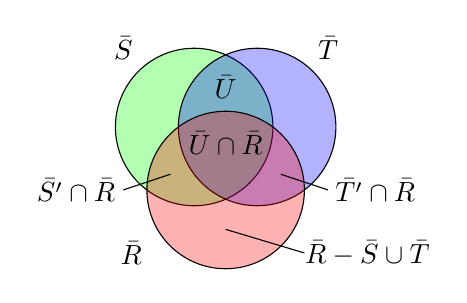
\begin{tikzpicture}
            \begin{scope} [fill opacity = .3]
            \draw[fill=green, draw = black] (-0.4,0.3) circle (1);
            \draw[fill=blue, draw = black] (0.4,0.3) circle (1);
            \draw[fill=red, draw = black] (0,-0.5) circle (1);
            \end{scope}
            \node at (-1.3,1.3) {\textbf{$\bar{S}$}};
            \node at (1.3,1.3) {\textbf{$\bar{T}$}};
            \node at (-1.2,-1.3) {\textbf{$\bar{R}$}};
            \node at (0,0.8) {\textbf{$\bar{U}$}};
            \node at (0,0.1) {\textbf{$\bar{U}\cap \bar{R}$}};
            \node at (-1.9,-0.5) {\textbf{$\bar{S'}\cap \bar{R}$}};
            \node at (1.9,-0.5) {\textbf{$\bar{T'}\cap \bar{R}$}};
            \node at (1.8,-1.3) {\textbf{$\bar{R} - \bar{S} \cup \bar{T}$}};
            \coordinate (a) at (-1.3,-0.5);
            \coordinate (b) at (-0.7, -0.3);
            \draw (a) -- (b);
            \coordinate (c) at (1.3,-0.5);
            \coordinate (d) at (0.7, -0.3);
            \draw (c) -- (d);
            \coordinate (e) at (1,-1.3);
            \coordinate (f) at (0, -1);
            \draw (e) -- (f);
    \end{tikzpicture}
    \end{center}

    Let $|\bar{U} \cap \bar{R}| = k$, $0 \leq k \leq h$.  On the other hand, let $|\bar{S'} \cap \bar{R}| = k_1$ and $|\bar{T'} \cap \bar{R}| = k_2$. We have $k_1+k_2 \leq m-k$. $\bar{R}$ has $m-k-k_1-k_2$ elements left to pick. Since $|\bar{S} \cup \bar{T}| = h+2(m-h) = 2m - h$, we are picking the rest of $m-k-k_1-k_2$ members from $N -2m +h$ elements. Therefore, (\ref{inverse_ip_1}) can be written as
    \begin{align} \label{inverse_ip}
        \langle \bar{S}, \bar{T} \rangle = \sum_{\substack{0 \leq k \leq h \\ 0 \leq k_1+k_2 \leq m-k}} \underbrace{\binom{h}{k}}_{\bar{U} \cap \bar{R}} \underbrace{\binom{m-h}{k_1}}_{\bar{S'} \cap \bar{R}}\underbrace{\binom{m-h}{k_2}}_{\bar{T'} \cap \bar{R}}\underbrace{\binom{N-2m+h}{m-k-k_1-k_2}}_{\bar{R} - \bar{S}\cup \bar{T}}f(k+k_1)g(k+k_2).
    \end{align}
    The expression depends only on $h$. We added under-brackets to remind the readers which set the selection is based upon. Finally, $|\bar{U}| = h$ can only take values $0,1,\cdots, m$. The product matrix can have at most $m$ distinct values. This finishes the proof.
\end{proof}
With the lemma proved, we are ready to prove that the inverse also pertains the same structure as we claimed at the beginning of this section.
\begin{theorem}
    Let $C$ be the covariance matrix corresponding to $m$-flip local optimum. If $C$ is invertible, then $C^{-1}$ is a good matrix.
\end{theorem}
\begin{proof}
    By our definition and our computation in section \ref{sec_covariance}, $C$ is a good matrix with dimension $\binom{N}{m}$-by-$\binom{N}{m}$. Assume $A$ to be a good $\binom{N}{m}$-by-$\binom{N}{m}$ matrix, and $g(l)$ the value of its entries, $0 \leq l \leq m$.

    By lemma \ref{good_matrix_lemma}, the product $CA$ is also a good matrix, with at most $m+1$ distinct values, given by the formula in (\ref{inverse_ip}) for $h = 0,1,\cdots m$. We already know how to compute the covariance matrix in (\ref{covar_entry}). Each formula can be seen as a linear combination of $g(l)$. Denote the coefficients as $a_{ij}$, $0 \leq i,j \leq m$. Recall that in (\ref{inverse_ip}), the formula with $h=m$ gives the expression of the diagonal entries. Let $a_{mj}$ be the coefficients of that formula. Now we consider the following system of linear equations.
    \begin{align}
        \sum_{j}a_{ij}g(j) = \mathbbm{1}(i=m), i = 0, \cdots m.
    \end{align}
    If the above system has a unique solution, this means $A = C^{-1}$ by definition because the equations mean the product of $CA$ is 1 on the diagonal and zero elsewhere. We prove this claim by contradiction.
    
    Assume to the contrary that there is no solution. Then we consider the following system of linear equations:
    \begin{align}
        \sum_{j}a_{ij}g(j) = 0, i = 0, \cdots m.
    \end{align} 
    This system must have nonzero solutions. This means we have found a matrix $A$ such that $CA = 0$. However, $C$ is invertible and that gives us a contradiction. The claim holds and at least one set of solutions exists.

    Finally, since there exist solutions, we have $A = C^{-1}$, and it must be unique. The system has a unique solution, which concludes our proof. 
\end{proof}
Note that in the proof we did not use any facts of the covariance matrix besides it being good. Therefore, we have the following more general statement.
\begin{theorem}
    If a good matrix is invertible, its inverse is also a good matrix.
\end{theorem}
Again, we will use the case of 2-flip as an example to illustrate how to make use of the theorems we just proved.
\begin{example}
    Let $C$ be the covariance matrix of 2-flip local optimum. Let $f(l)$ be the value of its entries, $l = 0,1,2$. By lemma \ref{covar_lemma}, we have that 
    \begin{align}
        f(0) = 4, f(1) = N-2, f(2)=2(N-2).
    \end{align}
    Let $g(l), l=0,1,2$ be the values of $C^{-1}$'s entries. We have 3 unknown variables, and (\ref{inverse_ip}) gives us 3 equations for $h = 0,1,2$. Below are the equations:
    \begin{align}
        (N^2-7N+13)g(0)&       +(3N-10)g(1)+      g(2)=0, \nonumber \\
        (3N^2-19N+30)g(0)& +(N^2+2N-12)g(1)+ (N-2)g(2)=0, \nonumber \\
        (2N^2-10N+12)g(0)& +(2N^2-8N+8)g(1)+ (2N-4)g(2)=1.
    \end{align}
    The solutions are as follows:
    \begin{align}
        g(0) &= \frac{N^2-9N+16}{2(N^4-7N^3+2N^2+29N-16)}, \nonumber \\
        g(1) &= \frac{-N^3+12N^2-46N+56}{4(N^4-7N^3+2N^2+29N-16)}, \nonumber \\
        g(2) &= \frac{N^4-14N^3+74N^2-170N+144}{4(N^4-7N^3+2N^2+29N-16)}.
    \end{align}
    Then we can explicitly write down $C^{-1}$ for $m=2$ by using the definition of a good matrix. Moreover, we can see that asymptotically
    \begin{align}
        g(0) \to \frac{1}{2N^2}, g(1) \to -\frac{1}{4N}, g(2) \to \frac{1}{4}.
    \end{align}
\end{example}
\section{Computation of the Integral} \label{sec_integral}
Under Construction.
\bibliographystyle{plain}
\nocite{*}
\bibliography{citation}


\end{document}